\documentclass[journal]{IEEEtran}

\usepackage{graphicx}
\graphicspath{{../../../../Figures/}
	{../Figures/FactorPlots/}
	{../Images/PNG/}
	{../../../../Figures/GRSL_2020/}
	{../../../../Figures/GRSL_2020/FactorPlots/}
	{../../../../Images/GRSL_2020/}
	{../../../../Figures/Soybeans_231/}
}

\usepackage{subcaption}
\captionsetup[table]{font=small,size=smaller,textfont=sc}
\captionsetup[figure]{font=small,size=smaller}

\usepackage{booktabs}
\usepackage[T1]{fontenc}
\usepackage{cite}
\usepackage[cmex10]{amsmath}
%\usepackage{dblfloatfix}
\usepackage{url}
\usepackage{color}
\usepackage{bm,bbm}
\usepackage{wasysym}
\usepackage{siunitx}
\DeclareSIUnit\pertenmille{\text{\textpertenthousand}}
\usepackage{multirow,bigstrut}

\DeclareMathOperator{\Tr}{Tr}

\begin{document}

\title{Statistical Properties of Geodesic Roll-Invariant Indexes in PolSAR Data over Crops}

\author{Danilo~Fernandes,
	Debanshu~Ratha,
	Avik~Bhattacharya,~\IEEEmembership{Senior~Member,~IEEE},
	and~Alejandro~C.~Frery,~\IEEEmembership{Senior~Member,~IEEE}% <-this % stops a space
	\thanks{D.\ Fernandes is with the Instituto Federal de Alagoas, Brazil. Email: dfc@laccan.ufal.br}% <-this % stops a space
	\thanks{D.\ Ratha and A.\ Bhattacharya are with the \textit{Centre of Studies in Resources Engineering}
		-- CSRE, Indian Institute of Technology Bombay, Mumbai, India. Email: \{debanshu.ratha;avikb\}@csre.iitb.ac.in}% <-this % stops a space
	\thanks{A.\ C.\ Frery is with the School of Mathematics and Statistics, Victoria University of Wellington, 6140 New Zealand, and with the Key Lab of Intelligent Perception and Image Understanding of the Ministry of Education, Xidian University, Xi'an, China. Email: alejandro.frery@vuw.ac.nz}
	\thanks{Manuscript received XX; revised YY.}}

\markboth{IEEE Geoscience and Remote Sensing Letters}%
{D.\ Fernandes et al.\MakeLowercase{\textit{et al.}}: Statistics Geodesic Distances}

\maketitle

\begin{abstract}
We analyze from a statistical viewpoint roll-invariant geodesic features (Scattering Type Angle $\alpha_{\text{GD}}$, Helicity $\tau_{\text{GD}}$, and Purity $P_{\text{GD}}$), as measured on five dates of four different crops.
We show that the Beta distribution explains well both $\alpha_{\text{GD}}$ and $\tau_{\text{GD}}$, while the Hyperbolic distribution is a good model for $P_{\text{GD}}$.
These choices are guided by mapping third- and fourth-order sample statistics onto the Pearson System plane.
Finally, we make a temporal analysis of the behavior of these estimates.
\end{abstract}

\begin{IEEEkeywords}
	Geodesic distance, PolSAR, Kennaugh representation, geodesic roll-invariant indices
\end{IEEEkeywords}

\IEEEpeerreviewmaketitle

\section{Introduction}

\IEEEPARstart{P}{olarimetric}
data from extended targets are rich in valuable information.
An active research venue is the definition of features able to summarize such information leading to processing and analysis techniques.
The most useful features are the target roll-invariant parameters, i.e., those unaffected by the rotation of the target about the radar line of sight.

Among the most important polarimetric features, one should mention Cloude \& Pottier's $H/\alpha$ decomposition~\cite{CloudePottier:97}, and Touzi's roll-invariant target parameters~\cite{Touzi:TGARS:2007}.
They lead to successful target scattering classification procedures and geophysical parameter extraction.

More recently, Ratha et al.~\cite{APolSARScatteringPowerFactorizationFrameworkandNovelRollInvariantParametersBasedUnsupervisedClassificationSchemeUsingaGeodesicDistanceinpress}, using the notion of the geodesic distance ($\text{GD}$) on the unit sphere embedded in the $16$-dimensional real (Euclidean) space, obtained a set of roll-invariant parameters with which they built a PolSAR scattering classification scheme. 
The features derived by measuring the geodesic distances between PolSAR observation and elementary targets were useful in
change detection~\cite{ChangeDetectionPolSARGeodesicDistanceBetweenScatteringMechanisms},
unsupervised land-cover classification~\cite{ClassificationPolSARGeodesic}, 
vegetation monitoring~\cite{AGeneralizedVolumeScatteringModelBasedVegetationIndexfromPolarimetricSARData2019}, and 
extraction of urban footprint~\cite{NovelTechniquesforBuiltupAreaExtractionfromPolarimetricSARImages2019} using PolSAR images.
The geodesic distance also provides a radar vegetation index (CpRVI) for compact polarimetric data~\cite{ARadarVegetationIndexforCropMonitoringUsingCompactPolarimetricSARData}. 

However, the nature of these features is not deterministic, since they are extracted from extended targets and, thus, subjected to the influence of speckle.
Nevertheless, none of those above works has explored the features' statistical properties.

The first step in this direction was presented by Fernandes and Frery~\cite{StatisticalPropertiesofGeodesicDistancesBetweenSamplesandElementaryScatterersinPolSARImagery2019}.
The authors showed that Beta distributions adequately describe geodesic distances between samples and prototypes.
Such distances are the basis for computing the geodesic roll-invariant parameters, which, thus, inherit their stochastic nature.

In this paper, we perform a qualitative analysis of the three geodesic indices on samples from four crops and five dates.
By mapping third- and fourth-order statistics onto the Pearson System plane we find that both the Geodesic Scattering Type Angle and the Geodesic Helicity can be described by the Beta distribution.
There is no single distribution in that system able to describe the Geodesic Purity, but the mapping suggests the need of a four-parameter model.
We then verified that the Hyperbolic distribution, which has nice geometrical properties, is a good choice for these data.

Finally, we make a temporal analysis of the behavior of these estimates in the parameter space, and we verify that, collectively, they are able to discriminate among crops and dates.

This statistical knowledge is basilar for the design of, among others, classification algorithms based on roll-invariant parameters.

\section{Methodology}

\subsection{The Kennaugh Representation}

In PolSAR theory, the $2 \times 2$ complex scattering matrix $\bm S$ has
complete polarimetric information about backscattering
from targets:
$$
\bm S = \begin{bmatrix}
S_{\text{HH}} &S_{\text{HV}}\\
S_{\text{VH}} &S_{\text{VV}}
\end{bmatrix},
$$
where the subscripts $\text{H}$ and $\text{V}$ denote horizontal and vertical
polarizations, respectively. 
Following the reciprocity theorem
in the case of a monostatic radar, 
$S_{\text{HV}}=S_{\text{VH}}$.
In such case, we obtain the Pauli scattering vector as
$
\bm k = \frac1{\sqrt{2}}
\begin{bmatrix}
S_{\text{HH}} + S_{\text{VV}} 
& S_{\text{HH}} - S_{\text{VV}} 
& 2S_{\text{HV}}
\end{bmatrix}^T
$,
where $T$ denotes transposition.

The Pauli representation is useful for visual analysis (assigning its components to the red, green, and blue channels), and for defining the coherency matrix $\bm T$.
Consider the availability of $L$ measures over the same type of target, then
$$
\bm T = \begin{bmatrix}
T_{ij}
\end{bmatrix}_{1\leq i,j\leq 3}= \frac{1}{L} \sum_{\ell=1}^{n}\bm k_\ell \bm k_\ell^{T*},
$$
where ``$*$'' denotes the complex conjugate.

%Given a scattering matrix $\bm{S}$, the $4 \times 4$ real Kennaugh matrix $\bm{K}$ is defined as~\cite{Pottier09}:
%\begin{equation}
%	%\label{coKen}
%	\bm{K} = \frac{1}{2}\bm{A}^*(\bm{S} \otimes \bm{S}^*) \bm{A}^{*T}, \quad \bm{A} = 
%	\begin{bmatrix}
%		1 & 0 & 0 & 1\\
%		1 & 0 & 0 & -1\\
%		0 & 1 & 1 & 0\\
%		0 & j & -j & 0
%	\end{bmatrix},
%\end{equation}
%where $\otimes$ is the Kronecker product, and  $j = \sqrt{-1}$.
The Kennaugh matrix can be obtained from the coherency matrix $\bm{T}$~\cite{PolarisationApplicationsRemoteSensing}:
\begin{equation}
	\label{incoKen}
	\bm{K} =
\arraycolsep=.6pt
	\begin{bmatrix}
		\frac{T_{11}+T_{22}+ T_{33}}{2} & \Re(T_{12}) & \Re(T_{13}) & \Im(T_{23})\\
		\Re(T_{12}) & \frac{T_{11}+T_{22}-T_{33}}{2} & \Re(T_{23}) & \Im(T_{13})\\
		\Re(T_{13}) & \Re(T_{23}) & \frac{T_{11}-T_{22}+T_{33}}{2} & - \Im(T_{12})\\
		\Im(T_{23}) & \Im(T_{13}) & - \Im(T_{12}) &\frac{-T_{11}+T_{22}+T_{33}}{2}
	\end{bmatrix},
\end{equation}
where $\Re(\cdot)$ and $\Im(\cdot)$ denote real and imaginary parts of a complex number. 

The polarimetric nature of the target is preserved under the scaling of measurements. 
In this light, the unit normalized version of a Kennaugh matrix identifies the scattering class to which the observed Kennaugh matrix belongs.

The elements of $\bm{K}$ matrices lie on $\mathbbm{S}^{15}$, the surface of the unit sphere in $\mathbbm{R}^{16}$. 
Therefore, the geodesic distance is the natural way to measure the distance between the two $\bm{K}$ matrices and targets. 

The $\text{GD}$ between two $4 \times 4$ real Kennaugh matrices $\bm{K}_1$ and $\bm{K}_2$ is given in~\cite{APolSARScatteringPowerFactorizationFrameworkandNovelRollInvariantParametersBasedUnsupervisedClassificationSchemeUsingaGeodesicDistanceinpress} as
\begin{equation}
	\text{GD}(\bm{K}_1,\bm{K}_2) =  \frac{2}{\pi} \cos^{-1}\frac{\Tr(\bm{K}_1^T\bm{K}_2)}{\sqrt{\Tr(\bm{K}_1^T\bm{K}_1)}\sqrt{\Tr(\bm{K}_2^T\bm{K}_2)}} ,
	\label{eq:GD_Ken}
\end{equation}
where $\Tr$ denotes the trace operator. 
The factor $2/\pi$ normalizes the distance to $[0,1]$. 
Therefore, $\text{GD}$ is the distance between the projections of $\bm{K}_1$ and $\bm{K}_2$ on the unit sphere centered at the origin in the space of $4 \times 4$ real matrices. 
The $\text{GD}$ without the $2/\pi$ factor is an angular parameter (in radians) as it is computed over a unit sphere. 

The GD and associated measures have been successfully employed in several applications~\cite{ClassificationPolSARGeodesic,AGeneralizedVolumeScatteringModelBasedVegetationIndexfromPolarimetricSARData2019,NovelTechniquesforBuiltupAreaExtractionfromPolarimetricSARImages2019,APolSARScatteringPowerFactorizationFrameworkandNovelRollInvariantParametersBasedUnsupervisedClassificationSchemeUsingaGeodesicDistanceinpress,ChangeDetectionPolSARGeodesicDistanceBetweenScatteringMechanisms,ARadarVegetationIndexforCropMonitoringUsingCompactPolarimetricSARData}. Their statistical properties, however, have not been explored yet.

\subsection{Prototypes and Geodesic Measures}

The polarimetric backscattering response of prototypes provides a fundamental reference for the analysis and interpretation of PolSAR data.
The Kennaugh matrices used in this work are the 
Ideal Depolarizer (${\text{ID}}$),
{trihedral} ($\text{t}$),
and {left and right helixes (${\text{lh}}$, ${\text{rh}}$, respectively):
\begin{align*}
\bm{K}_{\text{ID}} & =
\begin{bmatrix}
1 & 0 & 0 & 0\\
0 & 0 & 0 & 0\\
0 & 0 & 0 & 0\\
0 & 0 & 0 & 0\\
\end{bmatrix},
&
\bm K_{\text{t}} &=
\begin{bmatrix}
1 & 0 & 0 & 0\\
0 & 1 & 0 & 0\\
0 & 0 & 1 & 0\\
0 & 0 & 0 & -1\\
\end{bmatrix}, \\
\bm K_{\text{lh}} &= 
\begin{bmatrix}
1 & 0 & 0 & -1 \\
0 & 0 & 0 & 0 \\
0 & 0 & 0 & 0 \\
-1 & 0 & 0 & 1\\
\end{bmatrix}
,
& \bm K_{\text{rh}} &=
\begin{bmatrix}
1 & 0 & 0 & 1 \\
0 & 0 & 0 & 0 \\
0 & 0 & 0 & 0 \\
1 & 0 & 0 & 1\\
\end{bmatrix}.
\end{align*}
Mandal et al.~\cite{ARadarVegetationIndexforCropMonitoringUsingCompactPolarimetricSARData} applied these and other matrices to crop monitoring using compact polarimetric SAR data.

%\begin{table}[hbt]
%	\centering
%	\caption{Kennaugh matrices of prototypes: {trihedral} ($\bm{K}_{\text{t}}$),
%		{cylinder} ($\bm{K}_{\text{c}}$),
%		{random volume} ($\bm{K}_{\text{rv}}$),
%		{dipole} ($\bm{K}_{\text{dp}}$),
%		{$+1/4$-wave} ($\bm{K}_{+1/4}$), 
%		{$-1/4$-wave} ($\bm{K}_{-1/4}$),
%		{narrow dihedral} ($\bm{K}_{\text{nd}}$),
%		{dihedral} ($\bm{K}_{\text{d}}$),
%		{left helix} ($\bm{K}_{\text{lh}}$), 
%		{right helix} ($\bm{K}_{\text{rh}}$), 
%		and Ideal Depolarizer ($\bm{K}_{\text{ID}}$)}\label{Tab:ElementaryK}
%	\setlength{\tabcolsep}{2.7pt}
%	\renewcommand{\arraystretch}{1.3}
%	\begin{tabular}{*{17}{c}}\toprule
%		&    \multicolumn{4}{c}{First Row} 
%		& \multicolumn{4}{c}{Second Row} 
%		& \multicolumn{4}{c}{Third Row} 
%		& \multicolumn{4}{c}{Fourth Row}\\ 
%		\cmidrule(rl){2-5} \cmidrule(rl){6-9} \cmidrule(rl){10-13} \cmidrule(rl){14-17} 
%		$\bm K_{\text{t}}$
%		& $1$ & $0$ & $0$ & $0$
%		& $0$ & $1$ & $0$ & $0$
%		& $0$ & $0$ & $1$ & $0$
%		& $0$ & $0$ & $0$ & $-1$ \\
%		$\bm K_{\text{c}}$
%		& $\frac{5}{8}$ & $\frac{3}{8}$ & $0$ & $0$
%		& $\frac{3}{8}$ & $\frac{5}{8}$ & $0$ & $0$
%		& $0$ & $0$ & $\frac{1}{2}$ & $0$
%		& $0$ & $0$ & $0$ & $-\frac{1}{2}$\\
%		$\bm K_{\text{rv}}$ 
%		& $1$ & $0$ & $0$ & $0$
%		& $0$ & $\frac{1}{2}$ & $0$ & $0$
%		& $0$ & $0$ & $\frac{1}{2}$ & $0$
%		& $0$ & $0$ & $0$ & $0$\\
%		$\bm K_\text{dp}$
%		& $1$ & $-1$ & $0$ & $0$
%		& $-1$ & $1$ & $0$ & $0$
%		& $0$ & $0$ & $0$ & $0$
%		& $0$ & $0$ & $0$ & $0$\\
%		$\bm K_{+1/4}$
%		& $1$ & $0$ & $0$ & $0$
%		& $0$ & $1$ & $0$ & $0$
%		& $0$ & $0$ & $0$ & $1$
%		& $0$ & $0$ & $1$ & $0$\\
%		$\bm K_{-1/4}$
%		& $1$ & $0$ & $0$ & $0$
%		& $0$ & $1$ & $0$ & $0$
%		& $0$ & $0$ & $0$ & $-1$
%		& $0$ & $0$ & $-1$ & $0$\\
%		$\bm K_{\text{nd}}$ 
%		&$\frac{5}{8}$ & $\frac{3}{8}$ & $0$ & $0$
%		& $\frac{3}{8}$ & $\frac{5}{8}$ & $0$ & $0$
%		& $0$ & $0$ & $-\frac{1}{2}$ & $0$
%		& $0$ & $0$ & $0$ & $\frac{1}{2}$\\
%		$\bm K_{\text{d}}$ &
%		$1$ & $0$ & $0$ & $0$
%		& $0$ & $1$ & $0$ & $0$
%		& $0$ & $0$ & $-1$ & $0$
%		& $0$ & $0$ & $0$ & $1$ \\
%		$ \bm K_{\text{lh}}$
%		& $1$ & $0$ & $0$ & $-1$
%		& $0$ & $0$ & $0$ & $0$
%		& $0$ & $0$ & $0$ & $0$
%		& $-1$ & $0$ & $0$ & $1$\\
%		$ \bm K_{\text{rh}}$
%		& $1$ & $0$ & $0$ & $1$
%		& $0$ & $0$ & $0$ & $0$
%		& $0$ & $0$ & $0$ & $0$
%		& $1$ & $0$ & $0$ & $1$\\
%		$\bm{K}_{\text{ID}}$
%		& $1$ & $0$ & $0$ & $0$
%		& $0$ & $0$ & $0$ & $0$
%		& $0$ & $0$ & $0$ & $0$
%		& $0$ & $0$ & $0$ & $0$ \\
%		\bottomrule
%	\end{tabular}
%\end{table}

Ratha et al.~\cite{APolSARScatteringPowerFactorizationFrameworkandNovelRollInvariantParametersBasedUnsupervisedClassificationSchemeUsingaGeodesicDistanceinpress} proposed three new roll-invariant geodesic parameters, in analogy with classical ones~\cite{CloudePottier:97,Touzi:TGARS:2007}: Scattering Type Angle, Helicity, and Purity.

The geodesic scattering type angle $\alpha_{\text{GD}}$ describes 
the distance to the trihedral prototype:
\begin{equation}
	\alpha_{\text{GD}}(\bm{K}) = \frac{\pi}{2}  \text{GD}(\bm{K},\bm{K}_{\text{t}}).
\end{equation}

The helicity parameter provides a quantitative estimation of target symmetry~\cite{Touzi:TGARS:2007} in the observation. 
This quantity is derived as the (geometric) mean of the distances from left and right helices:
\begin{equation}
	\tau_{\text{GD}} = \frac\pi4 \big(1 - \sqrt{\text{GD}(\bm{K},\bm{K}_{\text{lh}})\text{GD}(\bm{K},\bm{K}_{\text{rh}})}\big).
\end{equation}
The multiplication by $\pi/4$ makes the scale equal (in radians) for comparison with $|\tau_{m_1}|$~\cite{Touzi:TGARS:2007}. 
For trihedral target, $\tau_{\text{GD}}' = 0$ and for helices $\tau_{\text{GD}}' = \pi/4$, which matches with the scattering at extremities of $|\tau_{m_1}|$.

The geodesic purity index measures the distance between a target and the ideal depolarizer, which is characterized by the $\bm{K}_{\text{ID}}$ matrix.
The geodesic purity index is then:
\begin{equation}
	P_{\text{GD}} = \Big(\frac{3}{2}\text{GD}(\bm{K}, \bm{K}_{\text{ID}})\Big)^2.
\end{equation}

We will analyze these three geodesic parameters:
purity, scattering type angle, and helicity, in their natural domains.
%, the two last without scaling, i.e., $\alpha_{\text{GD}}(\bm{K}) = \text{GD}(\bm{K},\bm{K}_{\text{t}})$, and 
%$\tau_{\text{GD}} = 1 - \sqrt{\text{GD}(\bm{K},\bm{K}_{\text{lh}})\text{GD}(\bm{K},\bm{K}_{\text{rh}})}$.
%With this, these two last measures lie in $[0,1]$.

\section{Statistical Description}

\subsection{Initial considerations}

Fernandes and Frery~\cite{StatisticalPropertiesofGeodesicDistancesBetweenSamplesandElementaryScatterersinPolSARImagery2019} showed that Beta distributions describe geodesic distances between carefully selected samples and prototypes.
They did not analyze the GD to the Ideal Depolarizer and, thus, there is no available information about the distribution of $P_{\text{GD}}$.

With those results in mind, on the one hand, one might expect that $\alpha_{\text{GD}}$ follows a Beta distribution.
On the other hand, the distribution of $\sqrt{XY}$, with $X$ and $Y$ Beta random variables, cannot be expressed, in general, in a simple form.
If these random variables are independent, which is unlikely our case, the distribution of their product involves the ${}_2F_{1}$ hypergeometric function~\cite[Corollary~2.1]{OntheDistributionoftheProductofIndependentBetaRandomVariables}.
Therefore, there is also no available information about the distribution of $\tau_{\text{GD}}$.

\subsection{Samples}

We analyzed five PolSAR images of the same region: the image from 16 May 2016, followed by four others at time intervals of $24$ days. 
The images are $30 \times 65$ pixels.
Figures~\ref{fig:day_0} to~\ref{fig:day_96} show the Canola data in Pauli Decomposition. 

\begin{figure}[hbt]
	\centering
	\subcaptionbox{16 May\label{fig:day_0}}{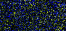
\includegraphics[width = .19\linewidth]{sb231_day_0}}
	\subcaptionbox{9 June\label{fig:day_24}}{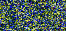
\includegraphics[width = .19\linewidth]{sb231_day_24}}
	\subcaptionbox{3 July\label{fig:day_48}}{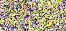
\includegraphics[width = .19\linewidth]{sb231_day_48}}
	\subcaptionbox{27 July\label{fig:day_72}}{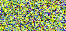
\includegraphics[width = .19\linewidth]{sb231_day_72}}
	\subcaptionbox{20 Aug.\label{fig:day_96}}{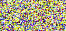
\includegraphics[width = .19\linewidth]{sb231_day_96}}
	\caption{Canola samples taken in 2016, in Pauli decomposition}
	\label{fig:sample_images}
\end{figure}

%Fig.~\ref{fig:AllIndexes} shows estimates of the densities of the three Geodesic Indices (Purity $P_{\text{GD}}$, Scattering Type Angle $\alpha_{\text{GD}}$, and Helicity $\tau_{\text{GD}}$) for the four crops (Canola, Oats, Soy Beans, and Wheat) in the five dates considered here.
%
%\begin{figure}[htb]
%	\centering
%	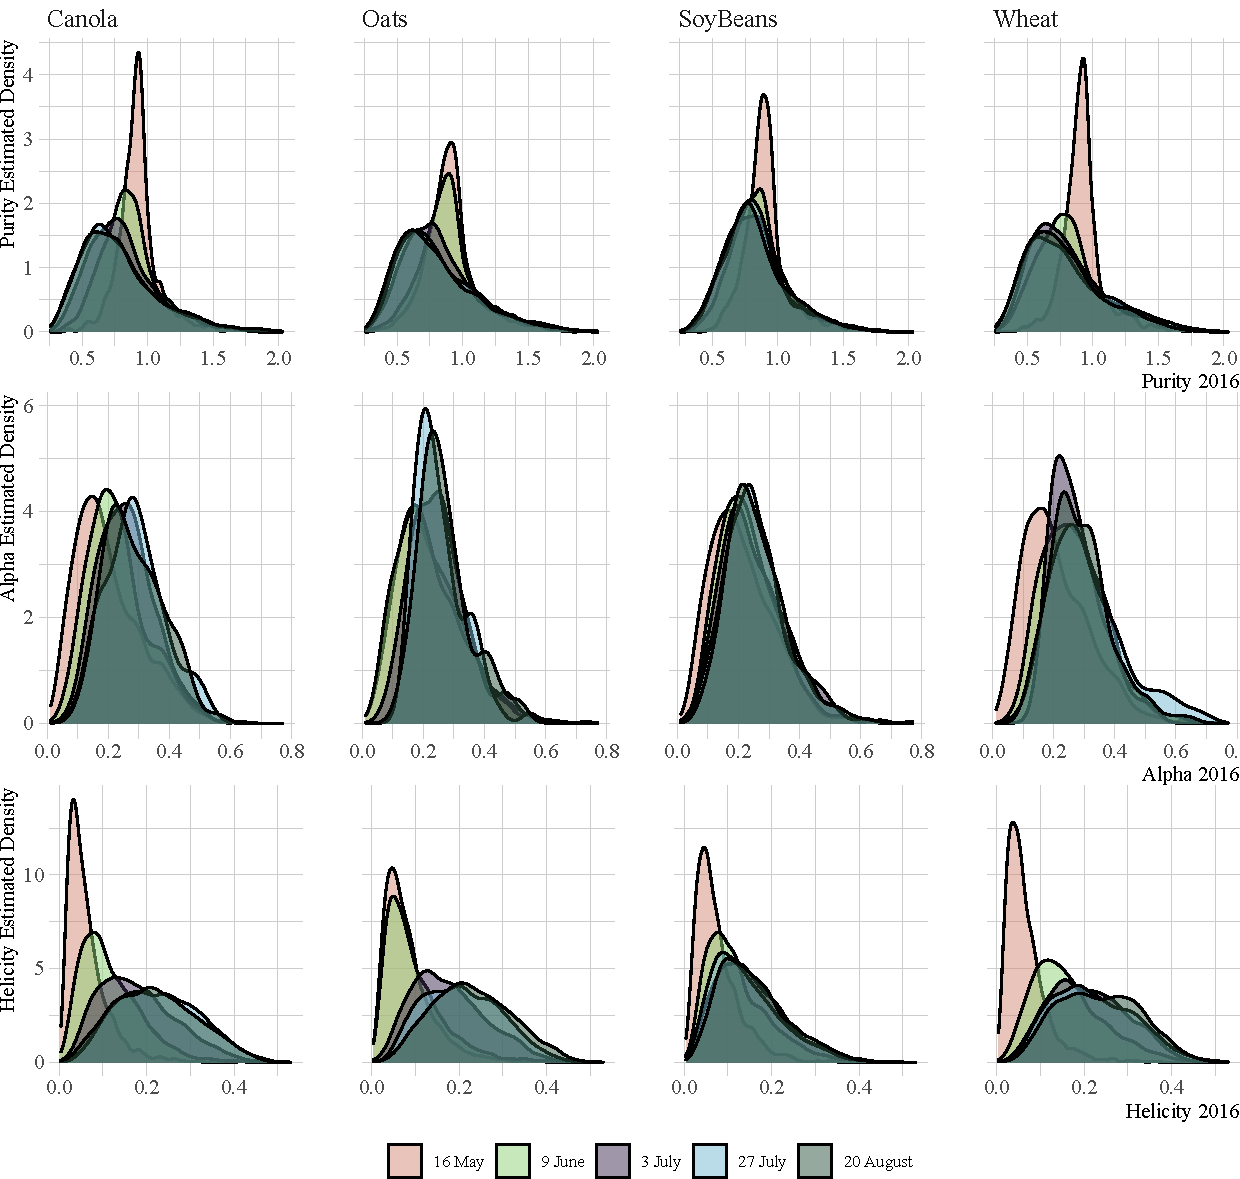
\includegraphics[width=\linewidth]{Indexes}
%	\caption{Density estimates of the three Geodesic Indices by crop and date.}\label{fig:AllIndexes}
%\end{figure}

\subsection{Choice of Models}

%\begin{table*}
%\centering
%\caption{Best fit within the Pearson System per Crop}
%\begin{tabular}{cccccccccccccr}
%\toprule
%& \multicolumn{3}{c}{Canola}
%& \multicolumn{3}{c}{Oats}
%& \multicolumn{3}{c}{SoyBeans}
%& \multicolumn{3}{c}{Wheat}\\
%\cmidrule(lr){2-4}
%\cmidrule(lr){5-7}
%\cmidrule(lr){8-10}
%\cmidrule(lr){11-13}
%\textbf{Type}
%& $\alpha_{\text{GD}}$
%& $\tau_{\text{GD}}$
%& $P_{\text{GD}}$
%& $\alpha_{\text{GD}}$
%& $\tau_{\text{GD}}$
%& $P_{\text{GD}}$
%& $\alpha_{\text{GD}}$
%& $\tau_{\text{GD}}$
%& $P_{\text{GD}}$
%& $\alpha_{\text{GD}}$
%& $\tau_{\text{GD}}$
%& $P_{\text{GD}}$
%& \textbf{Total}\\
%\cmidrule(lr){2-4}
%\cmidrule(lr){5-7}
%\cmidrule(lr){8-10}
%\cmidrule(lr){11-13}
%I 	&2 &3 &0 &0 &3 &0 &1 &3 &0 &1 &3 &1 & 17\\
%%II 	& & & & & & & & & & & & \\
%III &3 &1 &3 &4 &0 &2 &2 &1 &0 &3 &1 &2 & 22\\
%IV 	&0 &0 &2 &0 &0 &2 &0 &0 &3 &0 &0 &1 & 8\\
%V 	&0 &1 &0 &1 &0 &1 &2 &0 &2 &1 &0 &1 & 9\\
%VI 	&0 &0 &0 &0 &2 &0 &0 &1 &0 &0 &1 &0 & 4\\
%\cmidrule(lr){1-1}
%\cmidrule(lr){2-13}
%\cmidrule(lr){14-14}
%\textbf{Total} &5 &5 &5 &5 &5 &5 &5 &5 &5 &5 &5 &5 & 60\\ \bottomrule
%\end{tabular}
%\end{table*}

The Pearson system of distribution consists of those whose density $f$ has smoothness properties, and is the solution of
$$
\frac{df}{dx} = 
\frac{(x-a)f}{b_0+b_1 x + b_2 x^2}.
$$
This formulation gives rise to several types of distributions.
We are interested in six models which, in simplified form~\cite[Table~6, p.~45]{SystemsofFrequencyCurves}, are:
\begin{itemize}
	\item \textbf{Main Types:}
	\begin{itemize}
		\item \textbf{Type~I:} Beta distribution with density:
		\begin{equation}
		f(x; p, q) = \frac{\Gamma(p+q)}{\Gamma(p)\Gamma(q)} x^{p-1} (1-x)^{q-1} \mathbbm 1_{(0,1)}(x),
		\label{eq:BetaDensity}
		\end{equation}
		with $p,q>0$.
		
		\item \textbf{Type~IV:} the distribution characterized by the density
		\begin{align*}
		f(x&;\alpha,\lambda,\nu,m) =
		\frac{\Big|
			\frac{\Gamma(m+\imath\nu/2)}{\Gamma(m)}
			\Big|^2} {\alpha B(m-1/2,1/2)}\cdot\\
		%
	&	\Big[
		1+\Big(\frac{x-\lambda}{\lambda}
		\Big)^{2}
		\Big]^{-m} 
		% 
		\exp\Big\{-\nu\arctan\frac{x-\lambda}{\alpha}\Big\},
		\end{align*}
		where $\imath=\sqrt{-1}$,
		$B$ is the binomial coefficient,
		$\alpha>0$, 
		$m>1/2$, 
		and $\nu\neq0$.
		\item \textbf{Type~VI:} scaled and shifted F, or Beta Prime distribution with density:
		$$
		f(x;\alpha,\beta,\gamma,\lambda) = \frac{\Gamma(\alpha+\beta)}{|\gamma|\Gamma(\alpha) \Gamma(\beta)}
		\frac{
			\big(\frac{x-\lambda}{\gamma}\big)^{\alpha-1}
		}{
			\big(1+\frac{x-\lambda}{\gamma}\big)^{\alpha+\beta}
		},
		$$
		where $\alpha,\beta>0$, $\gamma\neq0$, and $(x-\lambda)/\gamma>0$.
		

	\end{itemize}
	\item \textbf{Transition Types:}
		\begin{itemize}
		\item \textbf{Type~II:} The distribution with density
	\begin{equation}
	f(x;\alpha,\beta) = k_{\alpha,\beta} \Big(
	1-\frac{x^2}{\alpha^2}
	\Big)^\beta \mathbbm 1_{(-\alpha,  \alpha)}(x),
	\label{eq:TypeIIDensity}
	\end{equation}
	with $\beta>-1$.

\item \textbf{Type~III:} Shifted Gamma distribution, with density:
$$
f(x; \alpha, \beta, \lambda)=
\frac{1}{|\beta|^\alpha \Gamma(\alpha)}
\big|x-\lambda\big|^{\alpha-1}
\exp\Big\{
-\frac{x-\lambda}{\beta}
\Big\},
$$
where $\beta\neq0$, $\alpha>0$, and $(x-\lambda)/\beta>0$.

		\item \textbf{Type~V:} shifted Inverse Gamma distribution, with density
$$
f(x;\alpha,\gamma,\lambda)= |\gamma|^\alpha \Gamma(\alpha) \big|x-\lambda\big|^{-\alpha-1} \exp\Big\{-\frac{\gamma}{x-\lambda} \Big\} ,
$$
where $\gamma\neq 0$, $\alpha>0$, and $\gamma/(x-\lambda)>0$.
\end{itemize}
\end{itemize}

We used the corrected Akaike Information Criterion (AICc) for model selection within the Pearson System of distributions.
This criterion provides a fair comparison of the fit of models with parameters of different dimension.
The best model is the one that minimizes
$$
\text{AICc}\big({\bm x; \mathcal D(\theta)}\big) =  -2 \ln \mathcal L\big(\widehat\theta\big) +  \frac{2 k n} {n-k-1}.
$$
where $\mathcal L$ is the likelihood under model $\mathcal D$,
$\theta$ is the parameter of dimension $k$ which indexes the model, $\widehat\theta$ is its maximum likelihood estimator,
and $n$ is the size of the sample $\bm x$.
Table~\ref{Tab:BestModelGeodesicIndex} shows the best model according to this criterion for each sample within the Pearson System.

\begin{table}[hbt]
	\centering
	\caption{Best Models per Geodesic Index according to the AICc criterion}\label{Tab:BestModelGeodesicIndex}
	\begin{tabular}{crrrr}
		\toprule
		\textbf{Type}
		& $\alpha_{\text{GD}}$
		& $\tau_{\text{GD}}$
		& $P_{\text{GD}}$ 
		& \textbf{Total}\\
		\cmidrule(lr){1-1}
		\cmidrule(lr){2-4}
		\cmidrule(lr){5-5}
		I	&18 &12 &1 	&31 \\
		II	&2 	&0 &0 	&2 \\
		III	&0 	&3 &7 	&10 \\
		IV	&0 	&0 &8 	&8 \\
		V	&0 	&1 &4 	&5 \\
		VI 	&0 	&4 &0 	&4 \\
		\cmidrule(lr){2-4} \cmidrule(lr){5-5}
			&20 &20 &20 & 60 \\
		\bottomrule
	\end{tabular}
\end{table}

The Pearson System also allows for a graphical display to assess the goodness-of-fit of a sample.
The Pearson plot depicts families of distributions in a plane with coordinates $(\beta_1,\beta_2)$, where $\beta_1$ is the square of the skewness, and $\beta_2$ is the kurtosis.

The plot shown in Fig.~\ref{Fig:PearsonPlanes} show where 
the Geodesic Scattering Type Angle $\alpha_{\text{GD}}$ (brown),
Geodesic Helicity $\tau_{\text{GD}}$ (blue),
and Geodesic Purity $P_{\text{GD}}$ (magenta)
are mapped into this plane.
Types~I, IV, and~VI distributions belong to the yellow, white, and purple areas, respectively.
Type~II lies in the vertical red segment, while Types~II and~V are limited to the red and purple lines, resp.
Other well-known distributions are shown as points, and the unfeasible region is depicted in gray.

\begin{figure}
\centering
\includegraphics[width=\linewidth]{PearsonPlotAlphaHelicityPurity}
	\caption{Samples Geodesic measures on the Pearson System plane: $\alpha_{\text{GD}}$ in brown, $\tau_{\text{GD}}$ in blue, and $P_{\text{GD}}$ in magenta.}\label{Fig:PearsonPlanes}
\end{figure}

Gathering the evidence provided by Table~\ref{Tab:BestModelGeodesicIndex} and by Fig.~\ref{Fig:PearsonPlanes}, and adding as additional criterion having a single model for $\alpha_{\text{GD}}$ and $\tau_{\text{GD}}$, we conclude that the Beta distribution is an adequate model.
The same information leads to no obvious choice for $P_{\text{GD}}$.

The samples of Geodesic Purity span distributions of Types~I (\SI{5}{\percent}),
III (\SI{35}{\percent}), 
IV (\SI{40}{\percent}), 
and~V (\SI{20}{\percent}).
Being the majority of samples well explained by Type~IV distributions, we expect to need a four-parameter model for $P_{\text{GD}}$.

Since there is no single law within the Pearson System able to describe $P_{\text{GD}}$, we turn our attention to the Hyperbolic distribution.
This model has been used with success in geology, fluid dynamics, biology, and econometry, to name a few~\cite{ErosionDepositionandSizeDistributionsofSand}.

The standard Hyperbolic distribution is characterized by the density
\begin{equation}
f(x;\pi,\zeta)=\frac{\exp\big\{-\zeta\big[\sqrt{(1+\pi^2)(1+x^2)} - \pi x \big]\big\}}{2 K_1(\zeta) \sqrt{1+\pi^2} }  
,\label{Eq:DensHyperbolic}
\end{equation}
where $K_1$ is the modified Bessel function of the third kind and order $1$, and $\zeta>0$ and $\pi\in\mathbbm R$ are shape parameters.
A location $\mu\in\mathbbm R$ and scale $\delta>0$  transformation yields the four-parameter Hyperbolic distribution, denoted $X\sim\text{H}(\mu,\delta,\pi,\zeta)$.
The parameters control the slopes of the two linear asymptotes of the log-density function.
The mode of~\eqref{Eq:DensHyperbolic} is located at $\mu+\delta\pi$, and the curvature of the log-density function at this point is $\delta^{-2}\zeta/(1+\pi^2)$;
this is a measure of the peakedness of the density at such point~\cite[vol~5, pp.~3278--3281]{EncyclopediaofStatisticalSciences}.


\subsection{Estimates}

In the subsequent analyses, all samples are of size $1950$. 

Table~\ref{tab:params_alpha} shows, for each crop type and date, 
the Maximum Likelihood estimates of the Beta model ($\widehat p,\widehat q$) for the Geodesic Scattering Type Angle $\alpha_{\text{GD}}$.

\begin{table}[hbt]
	\centering
	\caption{Maximum Likelihood estimates of the Beta model ($\widehat p,\widehat q$) for the Geodesic Scattering Type Angle $\alpha_{\text{GD}}$.}
	\label{tab:params_alpha}
	\setlength{\tabcolsep}{3.8pt}
	\begin{tabular}{clrrrrr}
		\toprule
		\textbf{Crop $\backslash$ Date} & & \textbf{16 May} & \textbf{9 June} & \textbf{3 July} & \textbf{27 July} & \textbf{20 Aug.}\\ \cmidrule{1-2} \cmidrule(lr){3-3} \cmidrule(lr){4-4} \cmidrule(lr){5-5} \cmidrule(lr){6-6} \cmidrule(lr){7-7}
		\textbf{Canola} 	
		& $\widehat{p}$ & 1.77     & 2.24      & 2.90      & 3.87      & 3.60 \\
		& $\widehat{q}$ & 4.47     & 3.26     & 2.68     & 2.47     & 2.38\\ 
		\midrule
		\textbf{Soy Beans} 
		& $\widehat{p}$ & 1.90      & 2.36      & 2.77      & 2.51      & 2.69 \\
		& $\widehat{q}$ & 4.23     & 3.33     & 3.15      & 3.11     & 2.89\\ 
		\midrule
		\textbf{Oats}
		& $\widehat{p}$ & 2.03       & 1.79      & 3.00      & 3.70      & 4.00 \\
		& $\widehat{q}$ & 4.09     & 3.03     & 2.72     & 2.48     & 2.35\\ 
		\midrule
		\textbf{Wheat}
		& $\widehat{p}$ & 1.87       & 2.74      & 3.69      & 3.78      & 3.93 \\
		& $\widehat{q}$ & 4.54     & 2.79     & 2.57     & 2.31     & 2.33\\
		\bottomrule
	\end{tabular}
\end{table}



Table~\ref{tab:params_helicity} shows the Maximum Likelihood estimates of the Beta model ($\widehat p,\widehat q$) for the Geodesic Helicity $\tau_{\text{GD}}$.

\begin{table}[hbt]
	\centering
	\caption{Maximum Likelihood estimates of the Beta model ($\widehat p,\widehat q$) for the Geodesic Helicity $\tau_{\text{GD}}$.}
	\label{tab:params_helicity}
	\setlength{\tabcolsep}{3.8pt}
	\begin{tabular}{clrrrrr}
		\toprule
		\textbf{Crop $\backslash$ Date} & & \textbf{16 May} & \textbf{9 June} & \textbf{3 July} & \textbf{27 July} & \textbf{20 Aug.}\\ \cmidrule{1-2} \cmidrule(lr){3-3} \cmidrule(lr){4-4} \cmidrule(lr){5-5} \cmidrule(lr){6-6} \cmidrule(lr){7-7}
		\textbf{Canola}     
		& $\widehat{p}$ & 2.19      & 2.68    & 3.39     & 4.41      & 3.89 \\
		& $\widehat{q}$ & 32.52     & 20.33     & 15.55  & 14.98     & 13.84\\ 
		\midrule
		\textbf{Soy Beans}
		& $\widehat{p}$ & 2.43       & 2.73       & 3.06       & 2.95       & 3.41 \\
		& $\widehat{q}$ & 30.10   & 19.81   & 17.18   & 17.77   & 18.26\\ 
		\midrule
		\textbf{Oats}
		& $\widehat{p}$ & 2.37       & 2.18      & 3.53     & 4.20     & 4.76 \\
		& $\widehat{q}$ & 26.53    & 20.41   & 16.49     & 16.11      & 15.95 \\ 
		\midrule
		\textbf{Wheat} 
		& $\widehat{p}$ & 2.35      & 3.34      & 4.39     & 4.20      & 4.68   \\
		& $\widehat{q}$ & 33.44   & 17.19   & 16.61   & 14.86   & 15.29   \\
		\bottomrule
	\end{tabular}
\end{table}

Table~\ref{tab:params_purity} shows the Maximum Likelihood estimates of the Hyperbolic model ($\widehat \mu,\widehat \delta, \widehat \pi, \widehat \zeta$) for the Geodesic Purity $P_{\text{GD}}$.

\begin{table}[hbt]
	\centering
	\caption{Maximum Likelihood estimates of Hyperbolic model ($\widehat \mu,\widehat \delta, \widehat \pi, \widehat \zeta$) for the Geodesic Purity $P_{\text{GD}}$.}
	\label{tab:params_purity}
	\setlength{\tabcolsep}{3.8pt}
	\begin{tabular}{clrrrrr}
		\toprule
		\textbf{Crop $\backslash$ Date} & & \textbf{16 May} & \textbf{9 June} & \textbf{3 July} & \textbf{27 July} & \textbf{20 Aug.}\\ \cmidrule{1-2} \cmidrule(lr){3-3} \cmidrule(lr){4-4} \cmidrule(lr){5-5} \cmidrule(lr){6-6} \cmidrule(lr){7-7}
		\textbf{Canola}     
		& $\widehat{\mu}$ & 0.907& 0.710& 0.019& 0.102 & 0.127\\
		& $\widehat{\delta}$ & 0.005& 0.192& 0.072& 0.030& 0.044  \\
		& $\widehat{\pi}$ &  0.098&  0.426&  9.371& 17.124& 10.973\\
		& $\widehat{\zeta}$ & 0.044& 1.733& 9.164& 5.190& 4.385\\
		\midrule
		\textbf{Soy Beans}
		& $\widehat{\mu}$ & 0.870& 0.680& 0.415& 0.570& 0.270 \\
		& $\widehat{\delta}$ & 0.012& 0.211& 0.345& 0.268& 0.372 \\
		& $\widehat{\pi}$ & 0.172& 0.482& 0.917& 0.633& 1.249 \\
		& $\widehat{\zeta}$ & 0.104& 2.065& 5.257& 3.015& 7.947 \\
		\midrule
		\textbf{Oats}
		& $\widehat{\mu}$ & 0.861& 0.818& 0.223& 0.153& 0.148 \\
		& $\widehat{\delta}$ & 0.042& 0.059& 0.271& 0.089& 0.037 \\
		& $\widehat{\pi}$ & 0.159&  0.254&  1.716&  5.541& 12.637 \\
		& $\widehat{\zeta}$ & 0.318& 0.375& 5.668& 4.548& 4.122 \\
		\midrule
		\textbf{Wheat} 
		& $\widehat{\mu}$ & 0.894& 0.293& 0.136& 0.153& 0.121 \\
		& $\widehat{\delta}$ & 0.006& 0.340& 0.056& 0.033& 0.027 \\
		& $\widehat{\pi}$ & 0.136&  1.253&  9.222& 13.940& 18.588 \\
		& $\widehat{\zeta}$ & 0.056& 6.135& 5.505& 3.670& 4.842 \\
		\bottomrule
	\end{tabular}
\end{table}

Fig.~\ref{Fig:PurityCanola16May} shows one of the most challenging Purity data sets: Canola, 16~May.
The histogram in linear scale (Fig.~\ref{Fig:HyperLinear}) resembles a Double Exponential distribution, but with different slopes.
The figure also shows the Hyperbolic density fitted with maximum likelihood estimates.
The quality of the fit is noticeable.
Since the geometric properties of the Hyperbolic distribution are designed in the logarithm of the probability density function, we also show the histogram and the fitted density in semilogarithmic scale (Fig.~\ref{Fig:HyperSemilog}).
We observed the quality of the fit not only for this data set, but for all the crops and dates here considered.

\begin{figure}[hbt]
\centering
\subcaptionbox{Histogram and Density in Linear Scale\label{Fig:HyperLinear}}{\includegraphics[width=.8\linewidth]{PurityCanola16May}}
\subcaptionbox{Histogram and Density in Semilogarithmic Scale\label{Fig:HyperSemilog}}{\includegraphics[width=.8\linewidth]{LogPurityCanola16May}}
\caption{Purity, Canola, 16~May, and fitted Hyperbolic density.}\label{Fig:PurityCanola16May}
\end{figure}

\section{Temporal Evolution}\label{Sec:TemporalEvolution}

Fig.~\ref{Fig:AlphaTemporal} shows the temporal variation of the estimates $(\widehat{p},\widehat{q})$ computed for the scattering type angle $\alpha_{\text{GD}}$ over each crop.

\begin{figure}[hbt]
	\centering
	\includegraphics[width=\linewidth]{AlphaTemporal}
	\caption{Temporal variation of $(\widehat{p},\widehat{q})$ for $\alpha_{\text{GD}}$.}\label{Fig:AlphaTemporal}
\end{figure}

Fig.~\ref{Fig:HelicityTemporal} shows the temporal variation of the estimates $(\widehat{p},\widehat{q})$ computed for the helicity $\tau_{\text{GD}}$ over each crop.

\begin{figure}[hbt]
	\centering
	\includegraphics[width=\linewidth]{HelicityTemporal}
	\caption{Temporal variation of $(\widehat{p},\widehat{q})$ for $\tau_{\text{GD}}$.}\label{Fig:HelicityTemporal}
\end{figure}

%We first checked the hypothesis that every pair of parameters from the same crop in different dates comes from different models.
%We used test statistics based on the Hellinger distance between the models~\cite{AnalyticExpressionsStochasticDistancesBetweenRelaxedComplexWishartDistributions}, and found that all the pairs are identifiable with \SI{5}{\percent} of significance, with the sole exception of $P_{\text{GD}}$ from Soy Beans in the two last dates.
%
%Fig.~\ref{fig:TemporalIndexes} (top) shows the temporal evolution of the parameter estimates $(\widehat\mu,\widehat\sigma)$ of the Lognormal distribution when describing the Geodesic Purity index $P_{\text{GD}}$.
%Canola, Oats, Soy Beans, and Wheat share similar behavior: $\widehat\mu$ decreases, while $\widehat\sigma$ increases with time, except for the two last dates of Canola and Wheat.
%The five stages of these four crops are easily identifiable using the Lognormal model, whereas Soy Beans have only four identifiable stages since, as noted, the estimates from the two last dates cannot be considered different.

Fig.~\ref{Fig:PCAPurityTemporal} shows the temporal variation of the two first principal components of the estimates $\widehat \mu,\widehat \delta, \widehat \pi, \widehat \zeta$ for the Geodesic Purity $P_{\text{GD}}$.
These two components capture, respectively, \SI{71.8}{\percent} and \SI{26.4}{\percent} of the variability of the estimates (approximately \SI{98.3}{\percent} of the total).

\begin{figure}[hbt]
\centering
\includegraphics[width=\linewidth]{HyperbolicPCATemporal}
	\caption{Temporal variation of the two first Principal Components of $\widehat \mu,\widehat \delta, \widehat \pi, \widehat \zeta$ for the Geodesic Purity $P_{\text{GD}}$.}\label{Fig:PCAPurityTemporal}
\end{figure}

In-situ measurements of the SMAPVEX16 campaign confirm that majority of the wheat and oat fields were at tillering during the second week of June. 
The Manitoba weekly crop reports~\cite{manitobaagriculture} suggest that soybean seeding finished during this period, and the plants were in their unifoliate to third trifoliate growth stage indicating very low Plant Area Index (a square meter of plant area per square meter ground; cf. Ref.~\cite{TheArchitectureofaDeciduousForestCanopyinEasternTennessee}) and biomass values. 
From the Manitoba weekly crop reports~\cite{manitobaagriculture}, canola seeding was almost completed, and the crop was emerging rapidly. 
Earlier seeded fields were reaching the rosette stage. 
Thus, the effect of the soil is expected to dominate the radar response rather than the vegetation component.
%Fig.~\ref{fig:TemporalIndexes} (middle) shows the temporal evolution of the parameter estimates $(\widehat p, \widehat q)$ of the Beta distribution when modeling the Geodesic Scattering Type $\alpha_{\text{GD}}$.
%Wheat is the crop where the estimates span most of the parametric space, as opposed to Soy Beans that gather around small values.
%Although all estimates are significantly different, the two first dates of Oats are very close.
During the first week of July, cereals (wheat and oats) were at their stem elongation to flag leaf stages. Some fields advanced to the heading stage. Consequently, we observe increases in PAI and biomass. 
In contrast, increases in PAI and wet biomass for soybean are less. 
According to the Manitoba weekly crop reports~\cite{manitobaagriculture}, the majority of canola fields were bolting, forming early flowers, whereas podding started in the most advanced fields.

The estimates $(\widehat p, \widehat q)$ of the Beta distribution for the Geodesic Helicity $\tau_{\text{GD}}$ (Fig.~\ref{Fig:HelicityTemporal}) suggest a decreasing tendency of $\widehat q$ along with an increasing trend of $\widehat p$ along time.
The second principal component of the estimates of the Hyperbolic distribution separates well the case where the estimates of the Beta distribution form a cluster: in Soybeans (Fig.~\ref{Fig:PCAPurityTemporal}). 

%\begin{figure*}
%	\centering
%	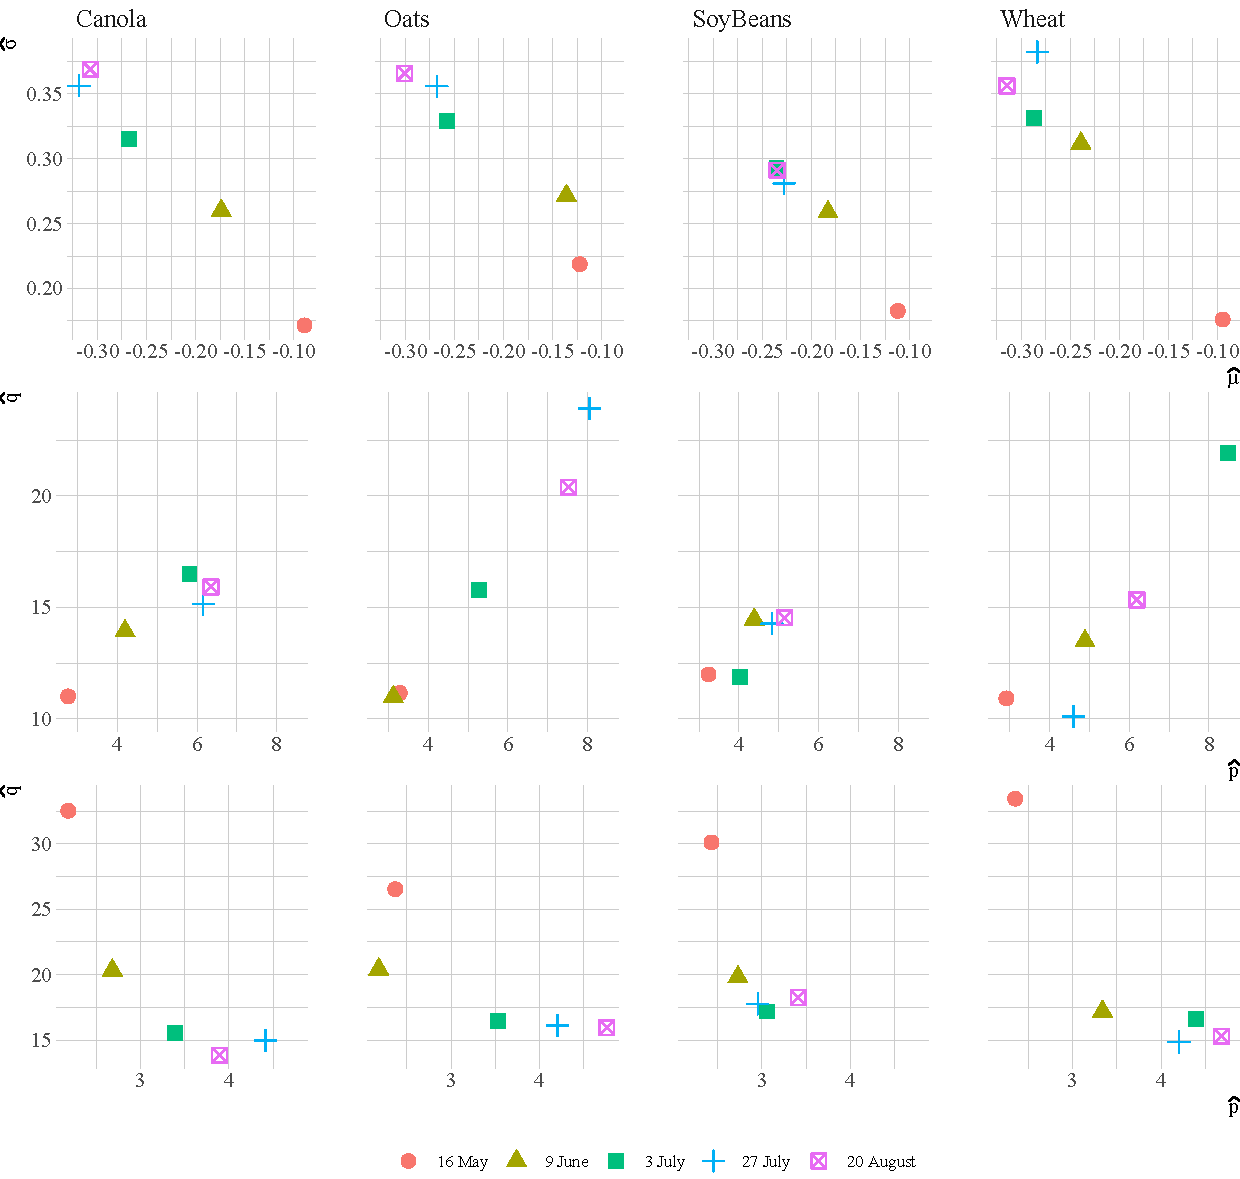
\includegraphics[width=\linewidth]{TemporalIndexes}
%	\caption{Temporal evolution of the parameter estimates $(\widehat\mu,\widehat\sigma)$ of the Lognormal distribution for the Geodesic Purity ($P_{\text{GD}}$, top), and of $(\widehat p,\widehat q)$ of the Beta distribution for the Geodesic Scattering Type Angle ($\alpha_{\text{GD}}$, middle) and Helicity ($\tau_{\text{GD}}$, bottom).}\label{fig:TemporalIndexes}
%\end{figure*}

\section{Conclusion}

Refs.~\cite{ClassificationPolSARGeodesic,
	AGeneralizedVolumeScatteringModelBasedVegetationIndexfromPolarimetricSARData2019,
	NovelTechniquesforBuiltupAreaExtractionfromPolarimetricSARImages2019,
	APolSARScatteringPowerFactorizationFrameworkandNovelRollInvariantParametersBasedUnsupervisedClassificationSchemeUsingaGeodesicDistanceinpress,
	ChangeDetectionPolSARGeodesicDistanceBetweenScatteringMechanisms,
	ARadarVegetationIndexforCropMonitoringUsingCompactPolarimetricSARData}
have shown the expressiveness and usefulness of indices derived from Geodesic Distances, but with no assessment of their statistical properties.
This paper shows that the three main Geodesic Indices (Geodesic Purity $P_{\text{GD}}$,
Geodesic Scattering Type Angle $\alpha_{\text{GD}}$, and
Geodesic Helicity $\tau_{\text{GD}}$) can be described by the Beta and Hyperbolic models.

The Hyperbolic distribution well describes Geodesic Purity.
The Beta distribution can model both the Geodesic Scattering Type Angle and the Geodesic Helicity.
These models are readily available in most statistical software.
The estimates are able to discriminate among dates of each crop.

%We used \texttt{R}~\cite{RManual} v.~3.6.3 for data processing and analysis (in particular, we used the functions provided by the \texttt{Rfast} library~\cite{Rfast} for parameter estimation), as well as for producing the graphical outputs (with the \texttt{ggplot2} library~\cite{ggplot2}).


\section*{Acknowledgment}

The authors would like to thank CNPq and Fapeal for providing partial support to this research. 
D.\ Ratha would like to acknowledge the support of CSIR, Government of India, towards his doctoral studies. 
The authors would like to thank Mr.\ Dipankar Mandal for providing information about the crop growth stages from the Manitoba (Canada) Agriculture reports.


\bibliographystyle{IEEEtran}
\bibliography{references}

\end{document}